\documentclass{beamer}

\usepackage{amssymb}
\usepackage{amsfonts}
\usepackage{amsmath}
\usepackage{amsthm}
\usepackage{setspace}
\usepackage{longtable}
\usepackage{graphicx}
\usepackage{mathtools}
\usepackage{color}
\usepackage{array}
\usepackage{calc} 
\usepackage{bm}
\usepackage{caption}
\usepackage{float}

\usetheme{CambridgeUS}
\useoutertheme{infolines}
%numbering
\setbeamercolor{background canvas}{bg=white}
\setbeamersize{text margin left=1cm,text margin right=1cm}

\title[AI1110  Assignment-10]{ASSIGNMENT-10}
\subtitle{AI1110}
\author[]{MUKUNDA REDDY \\ AI21BTECH11021}
\date

\begin{document}
  \begin{frame}
      \titlepage
  \end{frame}
  
  \begin{frame}{Outline}
      \tableofcontents
  \end{frame}
  
  \section{Question}
  \begin{frame}{Exercise 10-29}
     Show that the function
      $$ S(u,v) = H(e^{ju})H(e^{jv})H(e^{-j(u+v)}) $$
     is determined in terms of its values in the triangle of this figure.
     \begin{figure}
         \centering
         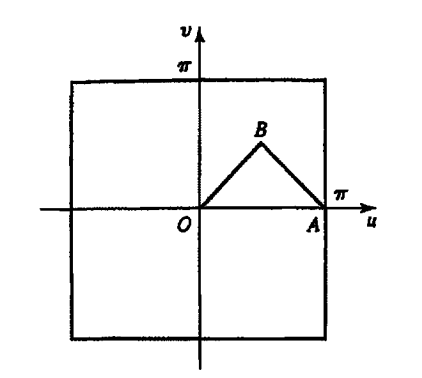
\includegraphics[scale=0.4]{fig1.png}
         \label{fig:my_graph}
     \end{figure}
  \end{frame}
  
  \section{Solution}
  \begin{frame}{Solution}
      We already know that
      \begin{equation}
      \label{1}
          S_a (u,v) = H_a (u)H_a (v)H_a (-ju-jv)  
      \end{equation}
     In this case clearly $S_a (u,v) = S(u,v)$
     for $|u|,|v|,|u+v|<\pi$ and 0 otherwise.The function
     $S_a (u,v)$ is a bispectrum of a bandlimited process, $x(t)$ with $\sigma = \pi$;
  \end{frame}
  
  \begin{frame}{Solution}
      hence it is determined from its values in the triangle of the figure.We already know that
      \begin{equation}
        S_{yyy} (u,v) = QH(u)H(v)H^{*}(u+v)  
       \end{equation}
       
      \begin{equation}
        S_{yyy} (u,v) = B(u,v)e^{j\theta (u,v)}
      \end{equation}
        the value of $H_a (w)$ is obtained from these equations.solving we get
      \[ 
        Where \: \: H_a (w) = 
      \begin{cases}
        $H(e^{jw})$ &, |w| \leq \pi \\
        0         &,  otherwise  \\
      \end{cases}
      \]
  \end{frame}
  
  \begin{frame}{Solution}
  Substituing the value $H_a (w)$  in
  \ref{1} we get required equation which we are interested to show that is \\
    $$ S(u,v) = H(e^{ju})H(e^{jv})H(e^{-j(u+v)}) $$
 
  \end{frame}
  
  
  
 \end{document}
